\begin{figure}[h]
	%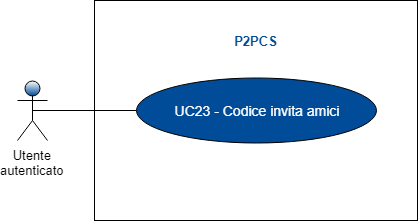
\includegraphics[width=8cm]{res/images/UC23Codiceamico.png}
	\centering
	\caption{Schema generale: codice invito amici}
\end{figure}
\subsubsection{UC23 - Codice invito amici}
\begin{itemize}
	\item \textbf{Attori Primari}: utente autenticato;
	\item \textbf{Descrizione}: agli utenti autenticati è reso disponibile un codice personale (composto da lettere e numeri) che può essere inviato ad un amico, non ancora registrato, per invitarlo ad usufruire dell'applicazione semplicemente inserendo questo "codice amico" in fase di registrazione nell'apposito spazio facendo guadagnare così punti bonus al proprietario del codice;
	\item \textbf{Scenario principale}: l'utente visualizza, nella voce \textit{Gestione Profilo} [UC14], il codice personale da inviare ad amici;
	\item \textbf{Precondizione}: l'utente autenticato ha selezionato la voce \textit{Gestione Profilo} [UC14] dal menu dell'applicazione;
	\item \textbf{Post-condizione}: l'utente autenticato ha visualizzato il suo codice personale. 
\end{itemize} 
